% Poster DATN HK253-DATN-071 -- nội dung chuyển từ bản PowerPoint A1.
\documentclass[final]{beamer}
\usepackage[orientation=portrait,size=a1,scale=1.06]{beamerposter}
\geometry{hmargin=1.8cm}

\usepackage[utf8]{inputenc}
\usepackage[vietnamese]{babel}
\usepackage[T5]{fontenc}
\usepackage{graphicx}
\usepackage{ragged2e}
\usepackage{tikz}
\usetikzlibrary{arrows.meta,positioning}

\usetheme{sharelatex}
\linespread{1.12}
\setlength{\parskip}{0.42em}

\definecolor{posterTeal}{RGB}{12,131,126}
\definecolor{posterBlue}{RGB}{52,126,255}
\definecolor{posterOrange}{RGB}{230,120,45}
\definecolor{posterLight}{RGB}{236,244,248}
\setbeamercolor{block title}{fg=white,bg=color2}
\setbeamercolor{block body}{fg=black,bg=posterLight}
\setbeamercolor{block title alerted}{fg=white,bg=posterTeal}
\setbeamercolor{block body alerted}{fg=black,bg=posterTeal!10}
\setbeamertemplate{blocks}[rounded][shadow=false]
\setbeamerfont{normal text}{size=\large}
\setbeamerfont{block title}{size=\Large,series=\bfseries}
\setbeamerfont{block body}{size=\large}
\setbeamerfont{block title alerted}{size=\Large,series=\bfseries}
\setbeamerfont{block body alerted}{size=\large}
\setbeamerfont{caption}{size=\large}
\setbeamerfont{caption name}{size=\large}

\newcommand{\metriccard}[4]{%
  \begin{beamercolorbox}[wd=\linewidth,ht=4.15cm,dp=0.7cm,rounded=true,sep=0.38em,center]{block body}
    {\LARGE\bfseries #1}\par
    {\color{posterTeal}\bfseries\LARGE #2}\par
    {\Large\bfseries #3}\par
    {\normalsize #4}
  \end{beamercolorbox}%
}

\tikzset{
  flow/.style={draw=posterBlue!70!black,very thick,rounded corners=5pt,
    fill=posterBlue!8,minimum width=5.75cm,minimum height=4.1cm,
    text width=5.05cm,align=center,font=\Large\bfseries},
  service/.style={draw=posterTeal!75!black,very thick,rounded corners=5pt,
    fill=posterTeal!8,minimum width=7.55cm,minimum height=5.4cm,
    text width=6.7cm,align=center,font=\large},
  mainarrow/.style={-{Latex[length=4mm]},very thick,color=posterOrange}
}

\title[AI hỗ trợ quyết định. Dữ liệu nghiệp vụ giữ quyền kiểm soát.]{%
XÂY DỰNG TRỢ LÝ MUA SẮM ĐA PHƯƠNG TIỆN\\[0.25ex]
SỬ DỤNG RAG VÀ COMPUTER VISION}

\author{%
MĐT: HK253-DATN-071 \quad \textbullet \quad GVHD: ThS. Võ Thanh Hùng\\[0.2ex]
SVTH: Huỳnh Thái Minh Châu -- MSSV: 2210352}

\begin{document}
\begin{frame}[t]
\begin{columns}[t,totalwidth=\textwidth]

% Luồng đọc tự nhiên: 01--02 ở cột trái, 03--04 ở cột phải; 05 chạy toàn trang.
\begin{column}{0.485\textwidth}
\justifying

\section{01. VẤN ĐỀ GIẢI QUYẾT}

\begin{block}{Khoảng cách ngữ nghĩa}
Người mua biết nhu cầu nhưng không nhớ đúng tên hoặc từ khóa sản phẩm.
\end{block}

\begin{block}{Khoảng cách thị giác}
Người mua có ảnh tham khảo nhưng khó diễn tả chính xác kiểu dáng bằng lời.
\end{block}

\begin{block}{Mất ngữ cảnh hội thoại}
Các câu hỏi nối tiếp về màu, kích thước và giá dễ bị hiểu sai nếu được xử lý độc lập.
\end{block}

\begin{alertblock}{Mục tiêu}
Hiểu đồng thời \textbf{văn bản, hình ảnh và lịch sử trao đổi} để tìm đúng sản phẩm và ra quyết định nhanh hơn.
\end{alertblock}

\vspace{0.55cm}
\section{02. GIẢI PHÁP ĐỀ XUẤT}

\begin{center}
{\color{posterBlue}\Large\bfseries LUỒNG CHÍNH TỪ NHU CẦU ĐẾN HÀNH ĐỘNG}

\vspace{0.55cm}
\begin{tikzpicture}
  \node[flow] (input) {VĂN BẢN + ẢNH\\{\large + lịch sử}};
  \node[flow,right=0.72cm of input] (understand) {HIỂU Ý ĐỊNH};
  \node[flow,right=0.72cm of understand] (rag) {TRUY HỒI + RAG\\{\large có căn cứ}};
  \node[flow,right=0.72cm of rag] (action) {XEM -- GIỎ -- ĐẶT\\{\large qua hệ thống lõi}};
  \draw[mainarrow] (input) -- (understand);
  \draw[mainarrow] (understand) -- (rag);
  \draw[mainarrow] (rag) -- (action);
\end{tikzpicture}

\vspace{0.9cm}
{\color{posterBlue}\Large\bfseries KIẾN TRÚC RÚT GỌN -- TÁCH BIỆT TRÁCH NHIỆM}

\vspace{0.55cm}
\begin{tikzpicture}
  \node[service] (front) {{\Large\textbf{REACT + NGINX}}\\[0.3em]
    Nhập yêu cầu\\Hiển thị kết quả};
  \node[service,right=0.8cm of front] (ai) {{\Large\textbf{AI SERVICE}}\\[0.3em]
    Truy hồi $\cdot$ RAG\\Bộ nhớ hội thoại};
  \node[service,right=0.8cm of ai] (core) {{\Large\textbf{SPRING BOOT}}\\[0.3em]
    Giá $\cdot$ tồn kho\\Giỏ hàng $\cdot$ đơn hàng};
  \draw[mainarrow,<->] (front) -- (ai);
  \draw[mainarrow,<->] (ai) -- (core);
\end{tikzpicture}
\end{center}

\vspace{0.45cm}
\begin{block}{Nguyên tắc kiểm soát}
AI đề xuất từ dữ liệu truy hồi; \textbf{Spring Boot xác nhận dữ liệu hiện hành và thực thi nghiệp vụ}. Vì vậy câu trả lời có căn cứ nhưng giá, tồn kho và đơn hàng vẫn do hệ thống lõi kiểm soát.
\end{block}

\end{column}

\begin{column}{0.485\textwidth}
\justifying

\section{03. SẢN PHẨM HOÀN CHỈNH}

% Ba lát cắt thay cho toàn màn hình: chữ và thao tác chính lớn hơn khi in.
\begin{figure}
  \centering
  \begin{minipage}[t]{0.315\linewidth}
    \centering
    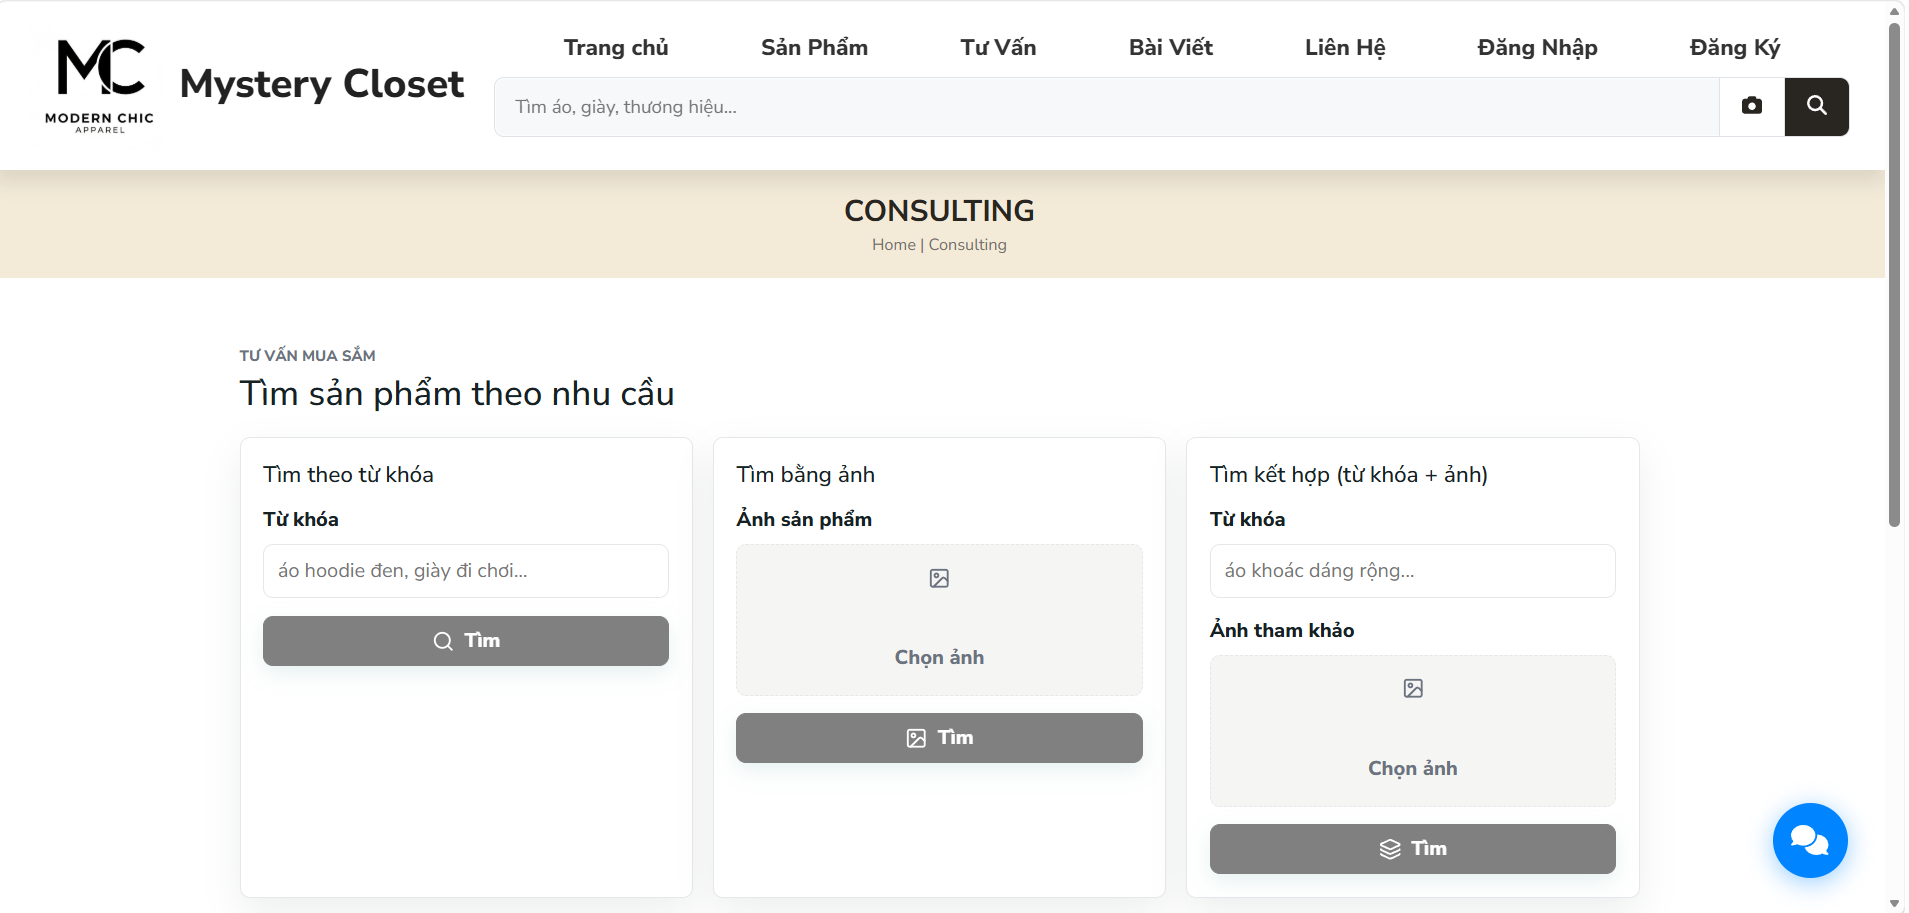
\includegraphics[width=\linewidth,trim=132 2 720 210,clip]{figures/search-ui.png}\par\vspace{0.3em}
    \colorbox{posterBlue}{\color{white}\strut\bfseries\quad VĂN BẢN\quad}
  \end{minipage}\hfill
  \begin{minipage}[t]{0.315\linewidth}
    \centering
    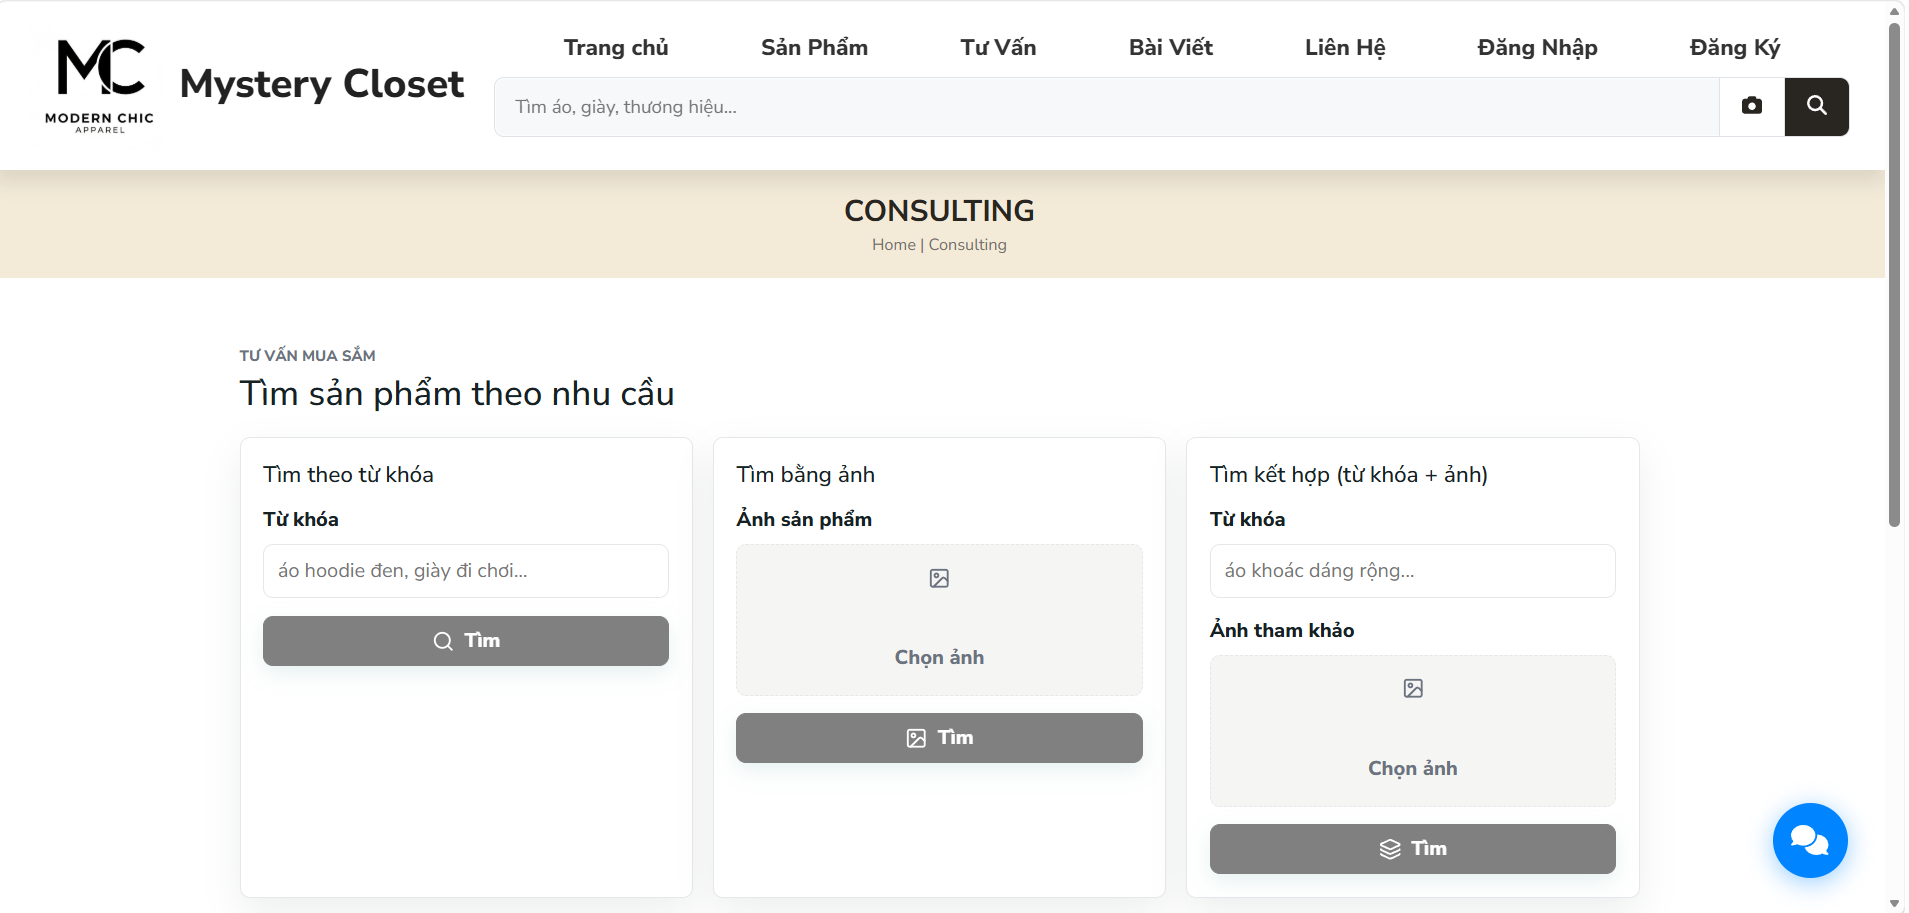
\includegraphics[width=\linewidth,trim=420 2 445 210,clip]{figures/search-ui.png}\par\vspace{0.3em}
    \colorbox{posterOrange}{\color{white}\strut\bfseries\quad HÌNH ẢNH\quad}
  \end{minipage}\hfill
  \begin{minipage}[t]{0.315\linewidth}
    \centering
    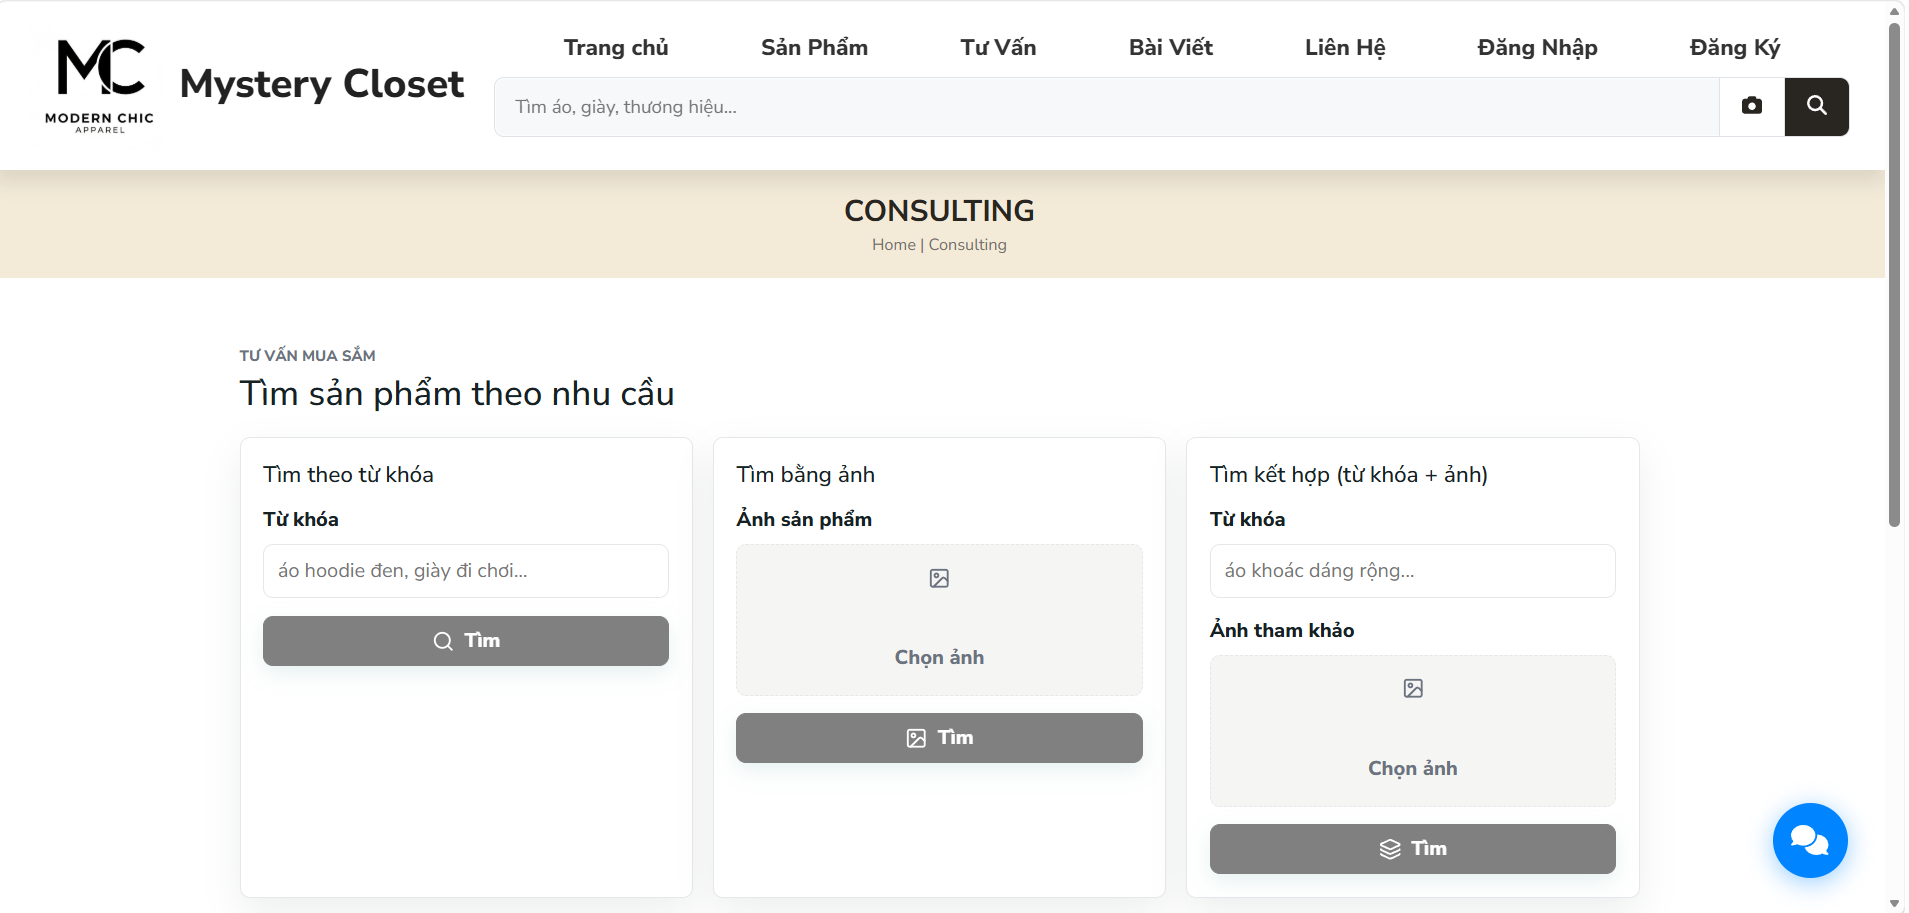
\includegraphics[width=\linewidth,trim=702 2 155 210,clip]{figures/search-ui.png}\par\vspace{0.3em}
    \colorbox{posterTeal}{\color{white}\strut\bfseries\quad KẾT HỢP\quad}
  \end{minipage}
  \caption{Ba đầu vào nổi bật: mô tả tự nhiên, ảnh tham khảo và truy vấn kết hợp.}
\end{figure}

\section{04. KẾT QUẢ NỔI BẬT}

% Lưới 2 cột x 3 hàng: mỗi cột là một nhóm kết quả, mọi thẻ cùng chiều cao.
\begin{center}
\begin{minipage}[t]{0.485\linewidth}
  \centering
  \colorbox{posterBlue}{\parbox{0.94\linewidth}{\centering\color{white}\Large\bfseries CHẤT LƯỢNG TRUY HỒI}}\par\vspace{0.55em}
  \metriccard{Hit@5}{100\%}{Text Search}{100 truy vấn}\par\vspace{0.55em}
  \metriccard{Exact Hit@5}{97\%}{Image Search}{100 ảnh bên ngoài}\par\vspace{0.55em}
  \metriccard{Strict Hit@5}{98\%}{Hybrid Search}{Image-conditioned; không rerank}
\end{minipage}\hfill
\begin{minipage}[t]{0.485\linewidth}
  \centering
  \colorbox{posterTeal}{\parbox{0.94\linewidth}{\centering\color{white}\Large\bfseries ĐỘ TIN CẬY HỆ THỐNG}}\par\vspace{0.55em}
  \metriccard{Rule-based Grounding}{100\%}{RAG + memory}{Context Precision 0,946; Recall 0,944}\par\vspace{0.55em}
  \metriccard{Backend tests}{102/102}{ca đạt}{Kiểm thử chức năng}\par\vspace{0.55em}
  \metriccard{AI regression}{430/430}{ca đạt}{Kiểm thử hồi quy}
\end{minipage}
\end{center}

\end{column}
\end{columns}

\vspace{0.55cm}
\section{05. TỪ TƯ VẤN ĐẾN HÀNH ĐỘNG}

\begin{columns}[T,totalwidth=\textwidth]
\begin{column}{0.61\textwidth}
  \begin{figure}
    \centering
    % Chỉ giữ câu hỏi, câu trả lời chính và hai gợi ý đầu tiên.
    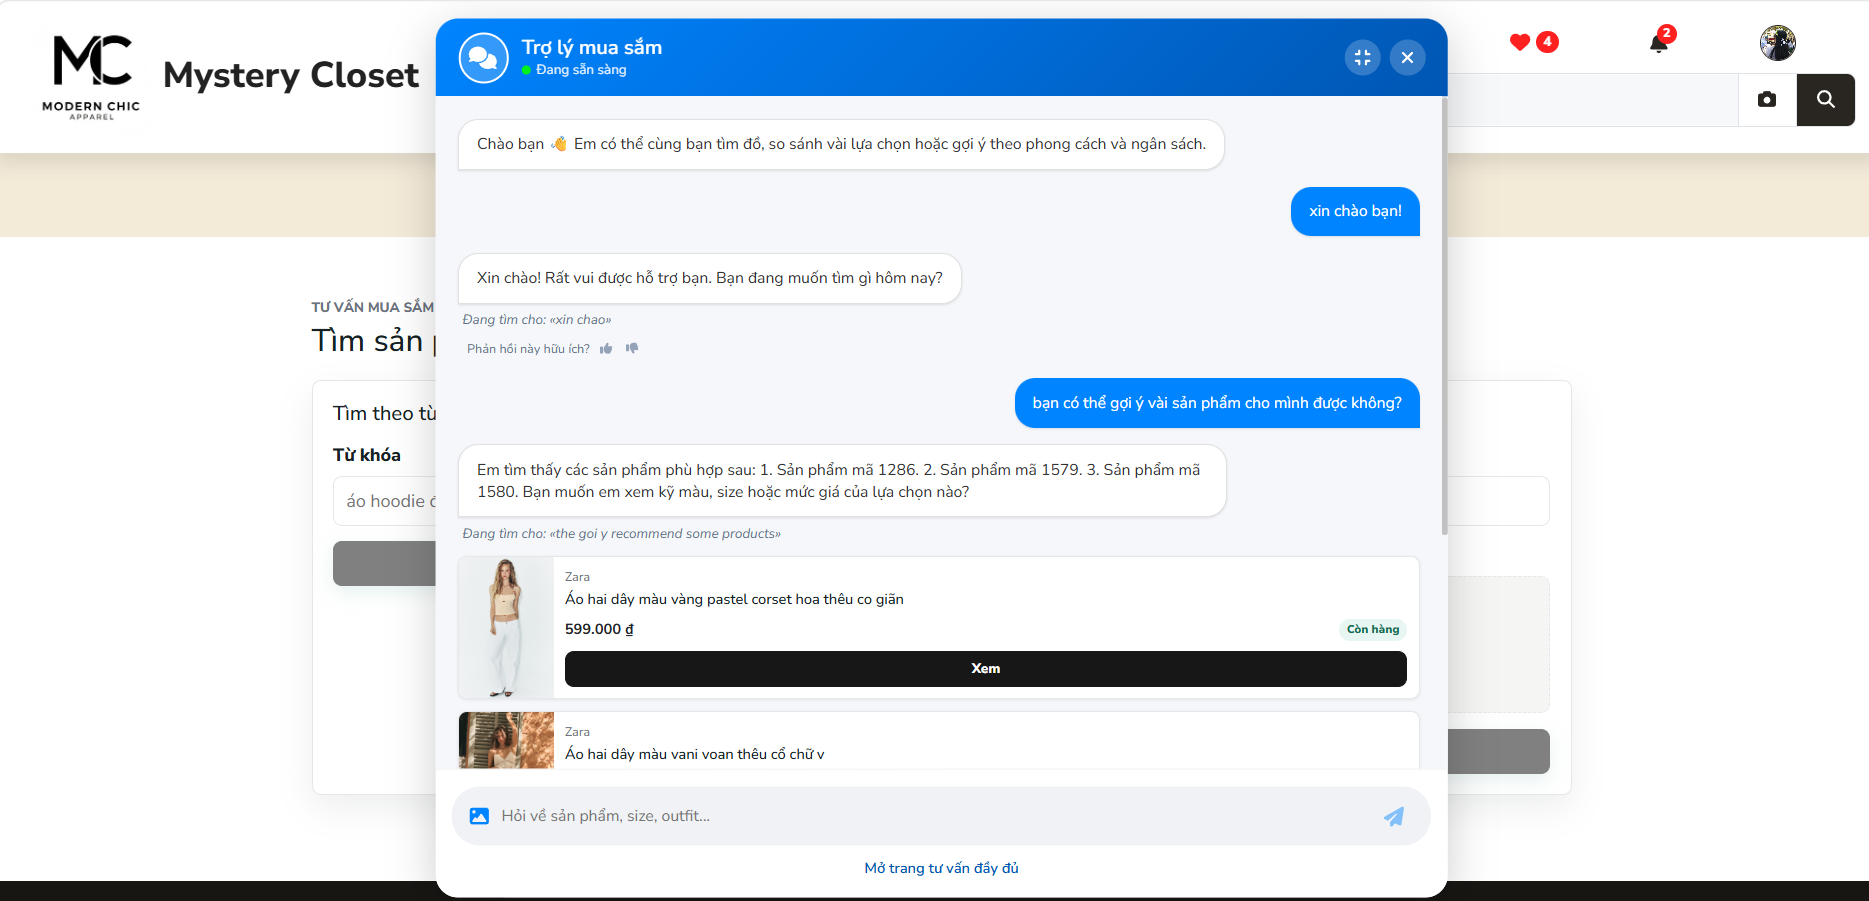
\includegraphics[width=0.98\columnwidth,trim=273 61 254 216,clip]{figures/chatbot-ui.png}
    \caption{\textbf{Đầu vào:} nhu cầu và câu hỏi nối tiếp. \textbf{Đầu ra:} câu trả lời có căn cứ kèm sản phẩm có thể mua ngay.}
  \end{figure}
\end{column}
\begin{column}{0.36\textwidth}
  \begin{block}{Đóng góp chính}
  \begin{itemize}
    \item Tìm kiếm đa phương thức trong một giao diện.
    \item Tư vấn RAG có căn cứ và bộ nhớ nhiều lượt.
    \item Tích hợp giỏ hàng, đặt hàng và quản trị.
    \item Đánh giá bằng baseline, ablation và kiểm thử hệ thống.
  \end{itemize}
  \end{block}

  \vspace{0.45cm}
  \begin{beamercolorbox}[wd=\linewidth,rounded=true,sep=0.65em]{block body}
    {\color{posterBlue}\Large\bfseries CÔNG NGHỆ}\par\vspace{0.3em}
    {\large\bfseries React $\cdot$ Spring Boot $\cdot$ FastAPI\\
    LangGraph $\cdot$ Qdrant $\cdot$ MySQL $\cdot$ Docker}
  \end{beamercolorbox}
\end{column}
\end{columns}

\vspace{2.5cm}
\begin{alertblock}{KẾT LUẬN}
\centering
{\LARGE\bfseries Tìm kiếm đa phương tiện và RAG giúp rút ngắn khoảng cách\\
từ nhu cầu tự nhiên đến hành động mua hàng.}
\end{alertblock}

\begin{center}
{\normalsize\textit{Phạm vi: snapshot 1.000 sản phẩm; benchmark chưa hoàn toàn held-out; tải AI và kiểm thử trên thiết bị thật còn giới hạn.}}
\end{center}
\end{frame}
\end{document}
